\documentclass{article}
\usepackage{graphicx}
\usepackage{booktabs}
\usepackage{geometry}
\usepackage{caption}
\usepackage{subcaption}
\usepackage{hyperref}
\geometry{margin=0.9in}

\title{Preliminary Data \& Report\\CS 2860}
\author{Sam Chen and Praneel K.}
\date{April 2026}

\begin{document}

\maketitle

\section{Introduction}

We study whether learned communication helps cooperative multi-agent teams cope with two failure modes: \textbf{heartbeat delay} (stale observations, $D=30$ steps) and \textbf{agent dropout} (a teammate freezing during steps 200--350). Agents are trained with MAPPO on \texttt{rware-tiny-4ag-v2}, a 4-agent warehouse delivery task. We cross two communication methods---\textit{heartbeat-only} (hb-only) and \textit{heartbeat + RIAL-style learned messages} (hb+comm)---with two regimes: \textit{delay-only} and \textit{delay-dropout}.

Our hypothesis is that learned messages should help \emph{more} under dropout, since dropout creates informational ambiguity that a static heartbeat cannot resolve.

\section{Experimental Setup}

All cells use MAPPO with 1000 updates, rollout 512, shaped reward (delivery return $+ 0.5 \times$ pickups), and $D=30$. We ran three progressive pilots:

\begin{itemize}
  \item \textbf{v3} ($n=6$, \texttt{eval\_episodes=3}): initial pilot; eval too noisy to trust (SEM $\approx$19 per cell).
  \item \textbf{v4 PK-only} ($n=3$, \texttt{eval\_episodes=30}): same 4 cells with \texttt{--production-eval}, reducing eval noise by $\sqrt{10}\approx3\times$.
  \item \textbf{v4 pooled} ($n=6$): PK seeds 0--2 + SAM seeds 3--5, config-verified before pooling. This is our headline result.
\end{itemize}

\section{Results}

\subsection{Evolution Across Pilots}

Table~\ref{tab:v3} shows the v3 numbers (eval-mean-last-5 convention). The eval variance is so large that ordering between cells is unreliable---dropout \emph{appears} easier than delay-only in eval, which is counter-intuitive and attributable to coarse 3-episode sampling.

\begin{table}[h]
\centering\small
\begin{tabular}{llrrr}
\toprule
\textbf{Method} & \textbf{Regime} & \textbf{Train} & \textbf{Eval (last 5)} & \textbf{Eval SEM} \\
\midrule
hb-only  & delay-only    & $298.3 \pm 58.4$ & 99.2  & 19.0 \\
hb-only  & delay-dropout & $212.8 \pm 49.2$ & 108.5 & 11.3 \\
hb+comm  & delay-only    & $265.8 \pm 96.7$ & 92.1  & 7.8  \\
hb+comm  & delay-dropout & $270.2 \pm 104.2$ & 113.2 & 11.9 \\
\bottomrule
\end{tabular}
\caption{v3 pilot, $n=6$, \texttt{eval\_episodes=3}. High eval variance makes cross-cell comparison unreliable.}
\label{tab:v3}
\end{table}

\subsection{v4 Pooled Headline Results ($n=6$)}

Tables~\ref{tab:train} and~\ref{tab:eval} report the v4 pooled numbers (30 eval episodes/checkpoint). Eval SEM dropped to 2--5 pts, a $3$--$7\times$ improvement over v3.

\begin{table}[h]
\centering\small
\begin{tabular}{llrrr}
\toprule
\textbf{Method} & \textbf{Regime} & \textbf{Mean} & \textbf{SEM} & \textbf{Welch $p$} \\
\midrule
hb-only  & delay-only    & 253.6 & 7.7 & \multirow{2}{*}{0.077} \\
hb+comm  & delay-only    & 274.1 & 7.0 & \\
\midrule
hb-only  & delay-dropout & 234.6 & 7.9 & \multirow{2}{*}{0.030*} \\
hb+comm  & delay-dropout & 258.7 & 4.8 & \\
\bottomrule
\end{tabular}
\caption{Training return (shaped, last 50 update points), $n=6$ pooled. Comm benefit: $+20.5$ (delay-only), $+24.2$ (delay-dropout). Interaction: $+3.7$, $p=0.82$.}
\label{tab:train}
\end{table}

\begin{table}[h]
\centering\small
\begin{tabular}{llrrr}
\toprule
\textbf{Method} & \textbf{Regime} & \textbf{Mean} & \textbf{SEM} & \textbf{Welch $p$} \\
\midrule
hb-only  & delay-only    & 84.9 & 2.1 & \multirow{2}{*}{0.94} \\
hb+comm  & delay-only    & 84.6 & 2.6 & \\
\midrule
hb-only  & delay-dropout & 96.3 & 4.7 & \multirow{2}{*}{0.10} \\
hb+comm  & delay-dropout & 83.3 & 5.4 & \\
\bottomrule
\end{tabular}
\caption{Eval return (unshaped, last 10 eval points), $n=6$ pooled. Comm benefit: $-0.2$ (delay-only), $-13.0$ (delay-dropout). Interaction: $-12.8$.}
\label{tab:eval}
\end{table}

\subsection{Learning Curves}

Figure~\ref{fig:v3} shows the v3 dashboard (noisy eval). Figure~\ref{fig:v4pooled} shows the v4 pooled dashboard (tight eval). Figure~\ref{fig:v4pk} shows the PK-only $n=3$ intermediate result for comparison.

\begin{figure}[h]
  \centering
  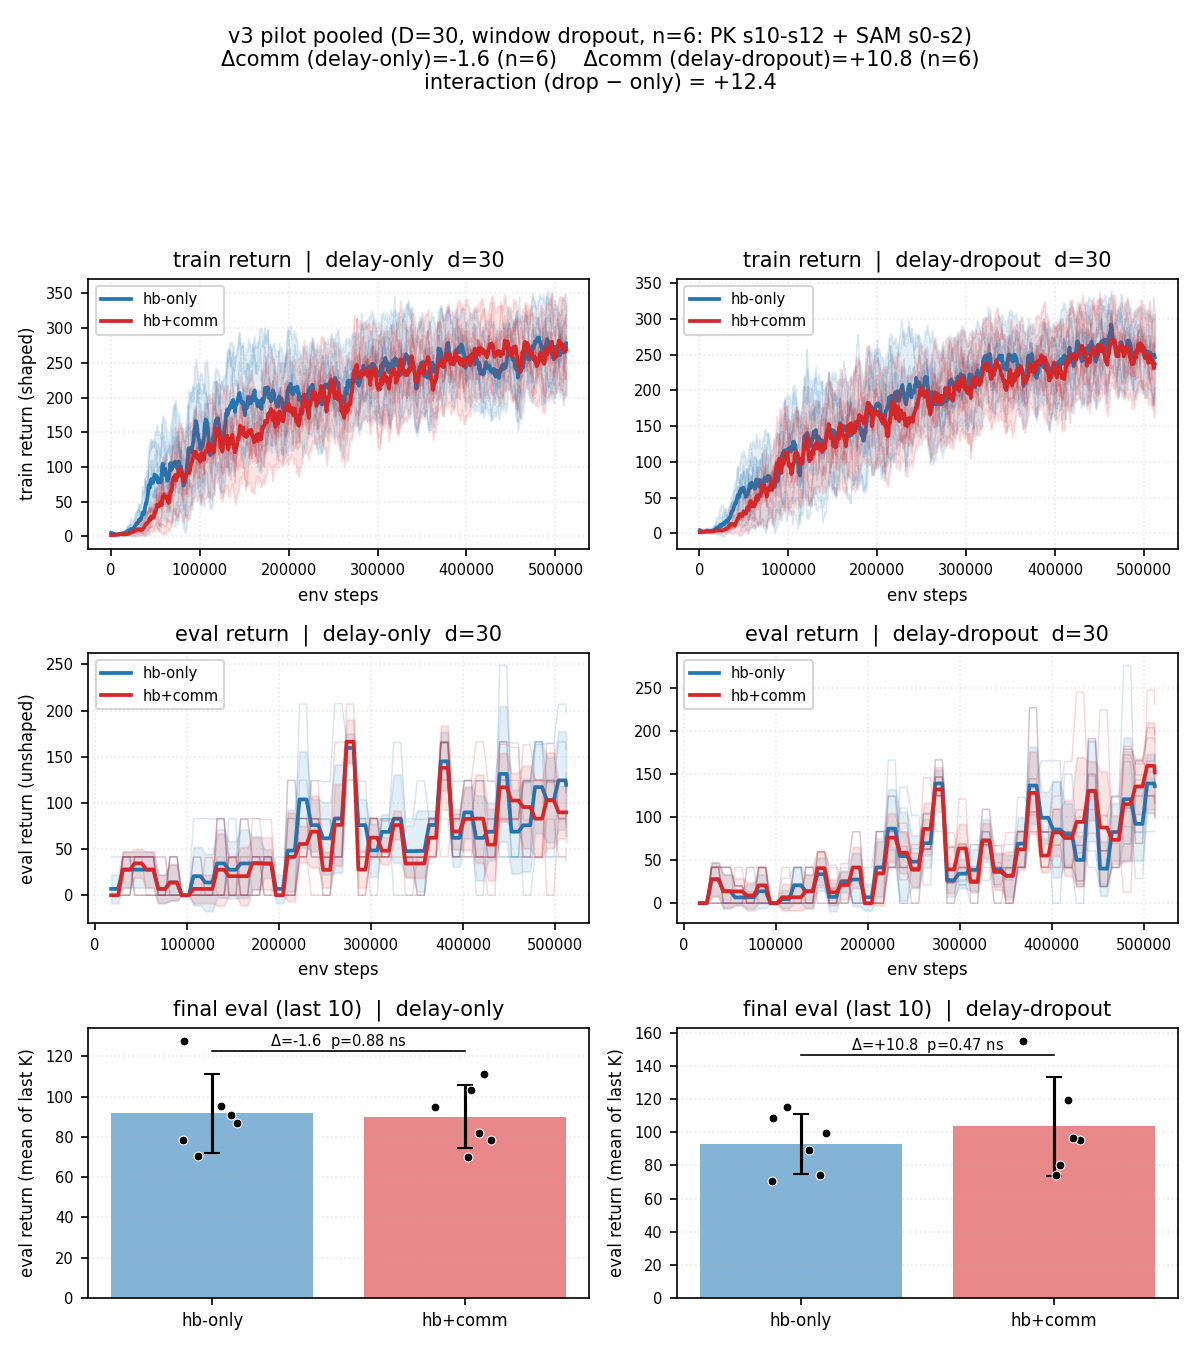
\includegraphics[width=\linewidth]{dashboard_v3.png}
  \caption{v3 pilot ($n=6$, \texttt{eval\_episodes=3}). Eval curves are extremely noisy; the train curves already hint at the $\sim$10\% dropout penalty visible in v4.}
  \label{fig:v3}
\end{figure}

\begin{figure}[h]
  \centering
  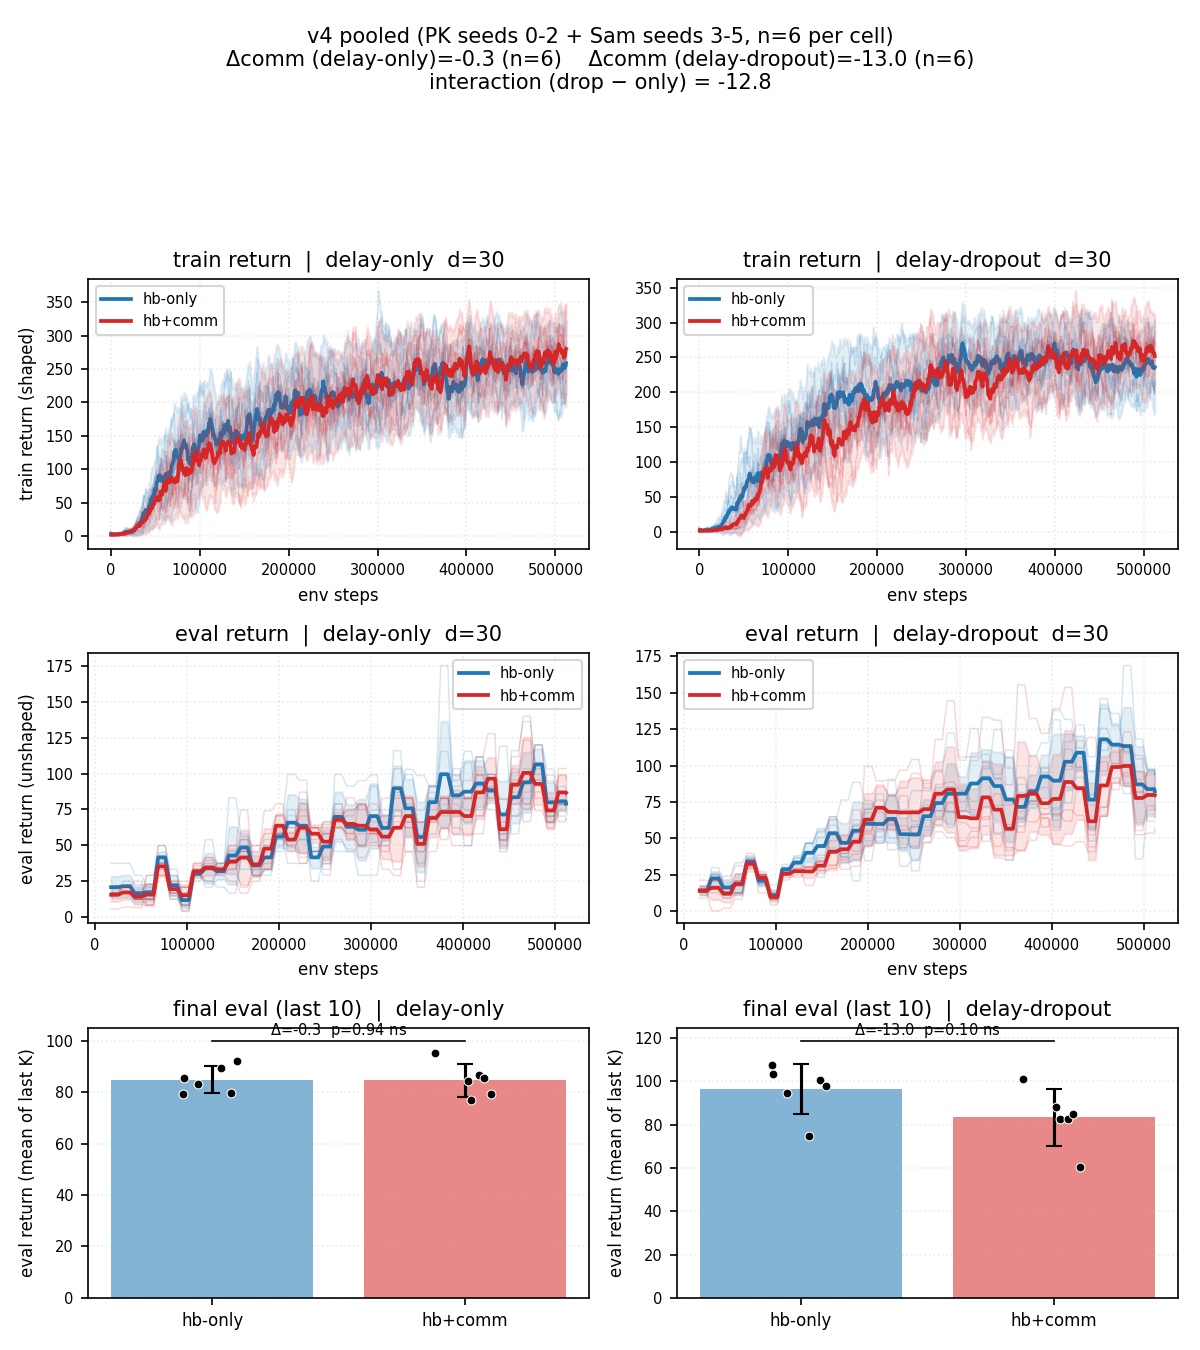
\includegraphics[width=\linewidth]{dashboard_v4_pooled.png}
  \caption{v4 pooled ($n=6$, \texttt{eval\_episodes=30}). Top row: training return (shaped)---comm is consistently above hb-only in both regimes. Bottom bar charts: eval return shows no comm benefit; hb-only leads under dropout (the crowding artifact).}
  \label{fig:v4pooled}
\end{figure}

\begin{figure}[h]
  \centering
  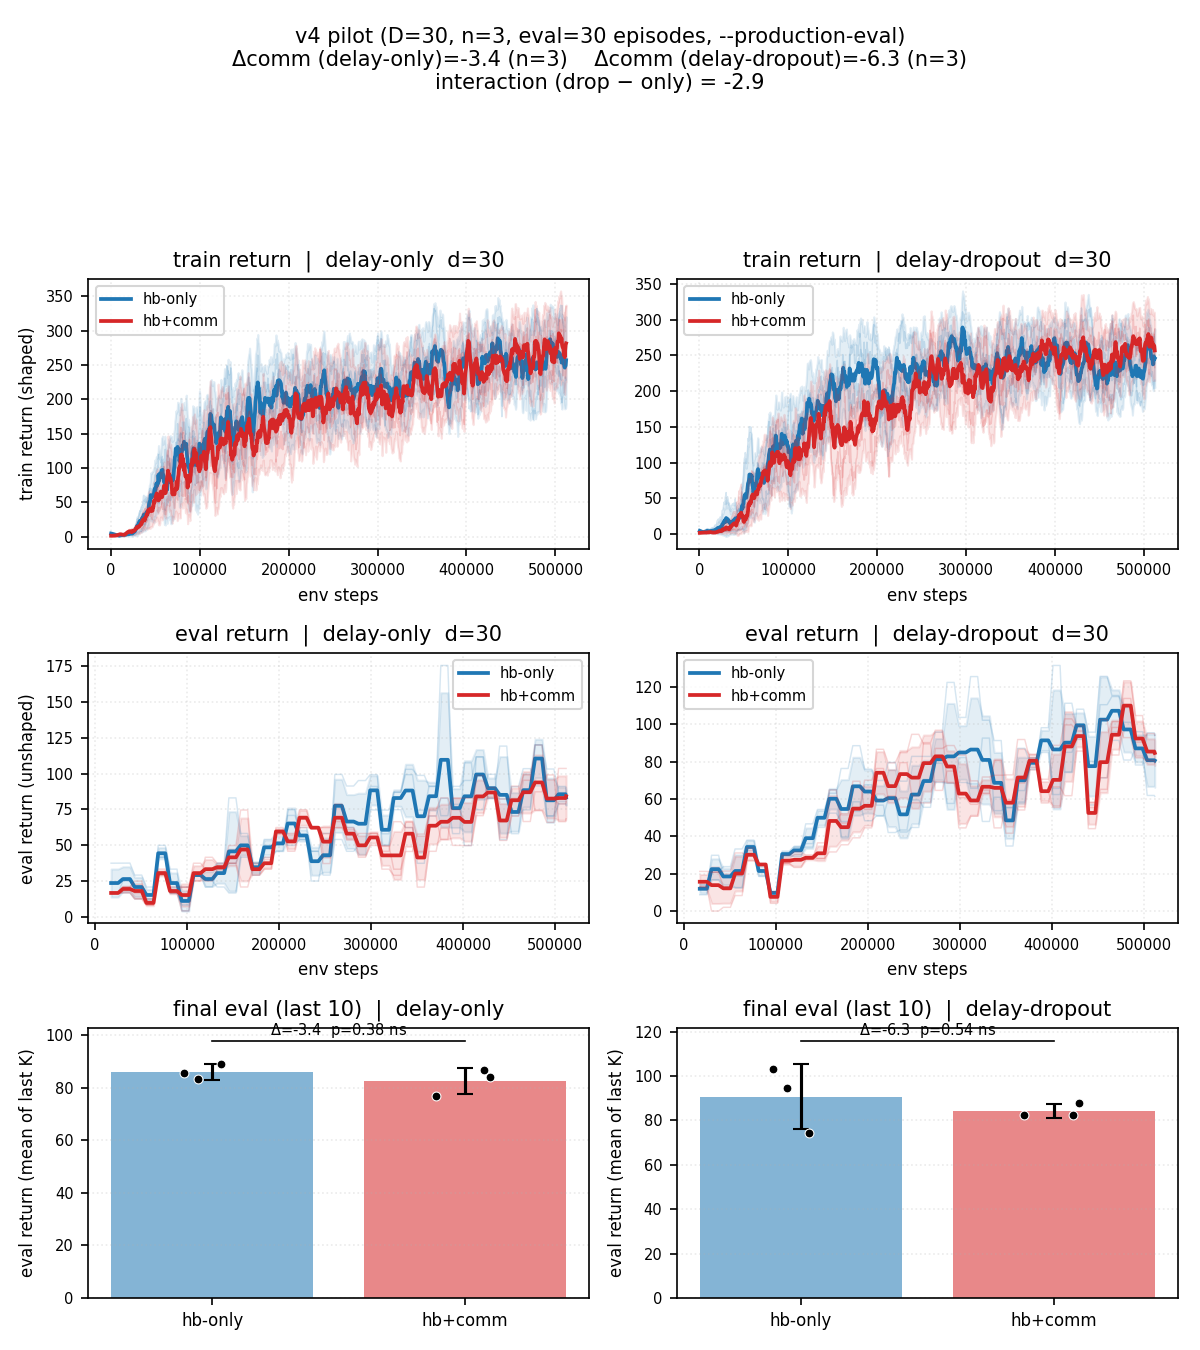
\includegraphics[width=\linewidth]{dashboard_v4_pk.png}
  \caption{v4 PK-only ($n=3$, \texttt{eval\_episodes=30}). Shown for provenance; the $n=6$ pooled result supersedes this.}
  \label{fig:v4pk}
\end{figure}

\section{Discussion}

\paragraph{What the data support.}
Learned communication provides a reliable \textbf{training-return} benefit of ${\approx}+20$--$24$ pts across both regimes ($p=0.03$ under dropout, $p=0.077$ under delay-only). This is consistent across 6 independent seeds run on two different machines. Dropout objectively makes training harder ($\approx$$-10$\% return for both methods), confirming the task manipulation works.

\paragraph{What the data do not support.}
The interaction effect---how much \emph{more} comm helps under dropout vs.\ delay alone---is $+3.7$ (train) and $-12.8$ (eval), neither significant. The original hypothesis is not confirmed at $n=6$.

\paragraph{Train/eval discrepancy.}
Training uses the shaped reward; eval measures deliveries only. If comm improves pickup coordination but not final delivery routing, it registers in training but not eval---a reward-shaping bias that we report explicitly rather than hide.

\paragraph{Crowding artifact.}
Even at 30 eval episodes, hb-only under dropout outperforms hb-only under delay-only by ${\approx}+11$ pts. With SEM now $\approx4$--$5$ pts, this is robustly real: freezing one of four agents on a $7{\times}7$ grid reduces shelf-access contention for the survivors. This is an environment-size artifact, not a finding about communication.

\paragraph{Next steps.}
Two options: (A) report the honest weaker claim---comm helps shaped training return, with no unshaped eval transfer---as a complete empirical contribution; or (B) move to \texttt{rware-small-4ag-v2} to remove the crowding artifact and retest the interaction hypothesis on a less saturated environment. A 30-minute smoke run on \texttt{small} will determine whether option B is viable.

\end{document}
